\documentclass[12pt]{article}

\usepackage[utf8]{inputenc}
%\usepackage[spanish]{babel}
\usepackage[spanish,es-tabla]{babel}
% Set page size and margins
% Replace `letterpaper' with `a4paper' for UK/EU standard size
% \usepackage[letterpaper,top=2cm,bottom=2cm,left=3cm,right=3cm,marginparwidth=1.75cm]{geometry}
\usepackage[a4paper,margin=1in]{geometry}
% Useful packages
\usepackage{amsmath}
\usepackage{graphicx}
\usepackage[colorlinks=true, allcolors=blue]{hyperref}

\usepackage{subcaption}
\usepackage{amssymb}
\usepackage{mathtools}
\usepackage[table,xcdraw]{xcolor}
\usepackage[backend=bibtex]{biblatex}
\usepackage{csquotes}
\usepackage{float}

\addbibresource{bibliografia.bib}


\begin{document}

% agregamos la caratula
\begin{titlepage}

\begin{center}
    
\includegraphics[width=5cm]{img/unc_logo.png} \hspace{2cm}
    
\includegraphics[width=5cm]{img/fcefyn_logo.jpg}
    \\[1cm]
    \vspace{5pt}
    \LARGE Universidad Nacional de Córdoba\\[0.6cm] 
    \large Facultad de Ciencias Exactas, Físicas y Naturales 
    \\[4cm] 
    \large Laboratorio N° 1
    \\[0.8cm]
    \large “AO Real: Errores”
    \\[0.2cm]
    \vspace{60pt}
    \begin{table}[!h]
    
    \centering
    \begin{tabular}{ll}
    \multicolumn{1}{c}{Integrantes} \\
    Britez, Fabio\\
    Corvalán, Abel \\
    Rodriguez, Facundo Nicolas 
    \end{tabular}
    \end{table}
    \vspace{20pt}
    \begin{table}[!h]
    \centering
    
    \begin{tabular}{ll}
    \multicolumn{1}{c}{Docente:} & Ing. Pablo Ferreyra
    \end{tabular}
    \end{table}
    \vfill
    Córdoba, República Argentina\\
    \today
\end{center}

\end{titlepage}
\newpage

% agregamos el indice
\tableofcontents
\newpage



\section{Introducción}
El objetivo es introducirse en el diseño, armado, medición y análisis de circuitos amplificadores lineales, teniendo en cuenta las fuentes de error del amplificador operacional real, y como se relacionan con las condiciones de entorno del circuito.

\subsection*{Metodología}

\begin{itemize}
\item[a.] Realizar una sintética introducción teórica. Amplificadores operacionales ideales y reales.
\item[b.] Analizar los circuitos sumadores propuestos, diseñar los circuitos en función del amplificador indicado y las condiciones de entorno. Debe presentar el desarrollo numérico, todos los cálculos analíticos, las mediciones y la simulación en PSPICE.
\item[c.] Analizar las condiciones de operación límite para el caso 1.A y 1.B en función de los errores del amplificador elegido y las condiciones de entorno.
\item[d.] Armar el circuito y hacer las mediciones en laboratorio.
\item[e.] Finalmente comparar los valores calculados, simulados y medidos, y extraer conclusiones cerca de las diferencias. Analizar las causas.
\end{itemize}



\section{Circuito: Amplificador sumador inversor}

El siguiente circuito es un un sumador. Debe ser diseñado para las condiciones de contorno especificadas más abajo.

\begin{figure}[h!]
    \centering
    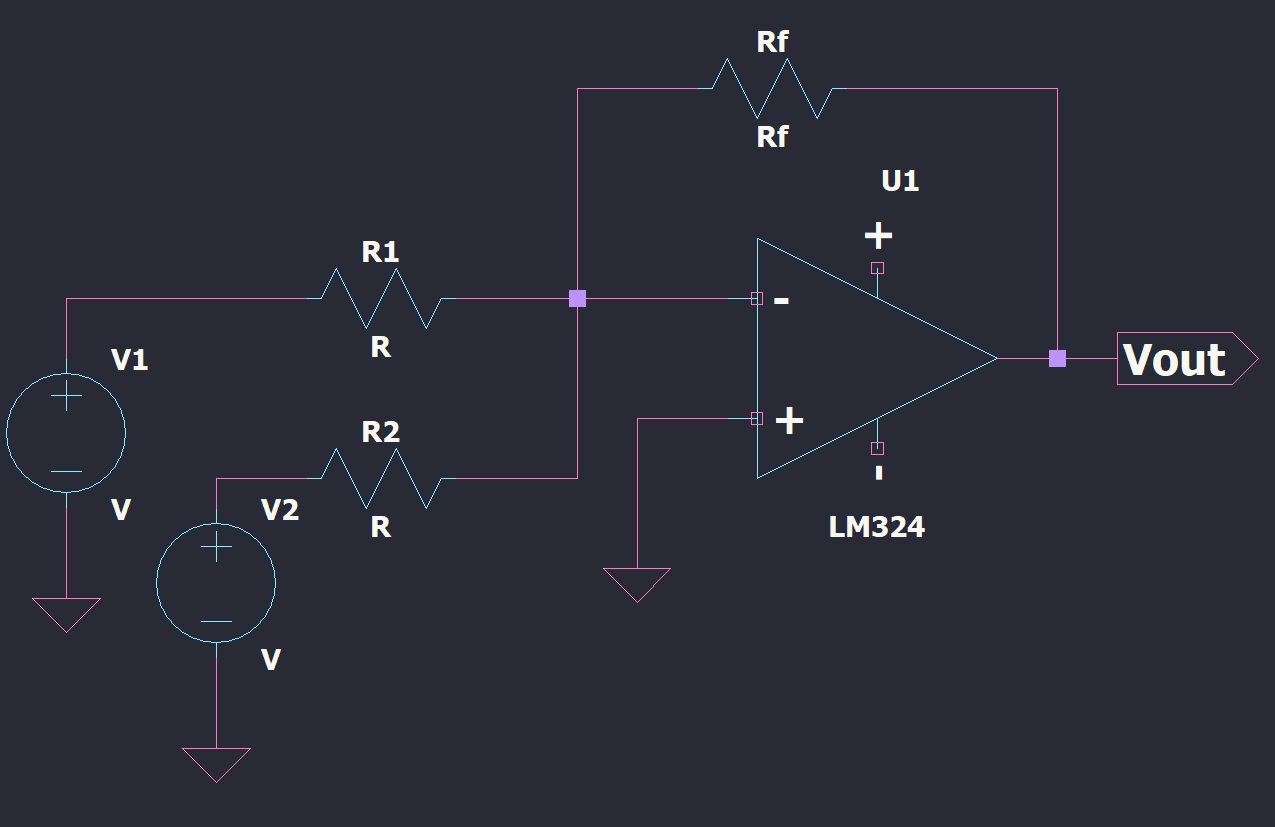
\includegraphics[width=0.90\linewidth]{img/esquematico_complete.png}
    \caption{Esquemático del circuito N° 1}
    \label{fig:esquematico}
\end{figure}

\begin{itemize}
  \item Tipo de amplificador operacional: LM324
  \item Alimentación: $Vcc = 10V, Vss = -10V$
  \item Ganancia en banda media: $A = \frac{V_O}{V_1} = \frac{V_O}{V_2} = 30$
  \item Impedancia de entrada: $Z_i$ del amplificador no puede alterar o cargar la fuente de señal, es decir, $R_i  \ll Zi_1$ y $Zi_2$ (al menos 10 veces)
  
  \item Resistencias: Usar Resistencias $<= 1M \Omega$
  \item Condiciones de las fuentes: Las fuentes V1 y V2 deben considerarse en las condiciones 1.A y 1.B

\end{itemize}





\section{Analisis del circuito}

\subsection{Vo = f(V1,V2)}

Este circuito tiene dos entradas, V1 y V2. 
La salida del circuito es la suma de las dos señales de entrada, amplificada. Para eso realizaremos el análisis haciendo uso del teorema de superposición nos permite calcular la respuesta de un circuito a dos o más señales de entrada, sumando las respuestas individuales a cada señal de entrada.

En este caso, podemos aplicar el teorema de superposición para calcular la salida del circuito como la suma de las salidas, considerando $V_2=0$ y luego considerando $V_1=0$. Para ambos casos podemos observar que tenemos un amplificador en configuración inversor. Por lo tanto considerando AO ideal: 

\vspace{1em}

Para el caso en el que pasivamos la fuente de tensión $V_2 = 0$ la tensión de salida es :

\[V_{01} = - \frac{R_f}{R} \cdot V_1 \]

Luego el caso en el que pasivamos la fuente de tensión $V_1 = 0$ obtenemos una tensión de salida:

\[V_{02} = - \frac{R_f}{R} \cdot V_2 \]

Aplicando el teorema, sumamos ambas salidas obtenemos:

\[V_{0} = V_{01} + V_{02} = - \frac{R_f}{R} \cdot (V_1 + V_2) \]

\vspace{1em}

\subsubsection{Ganancia del lazo: T}
Para calcular la ganancia T, primero pasivamos las fuentes de entrada y se abre el lazo, quedando así el siguiente circuito para analizar;

\begin{figure}[h!]
    \centering
    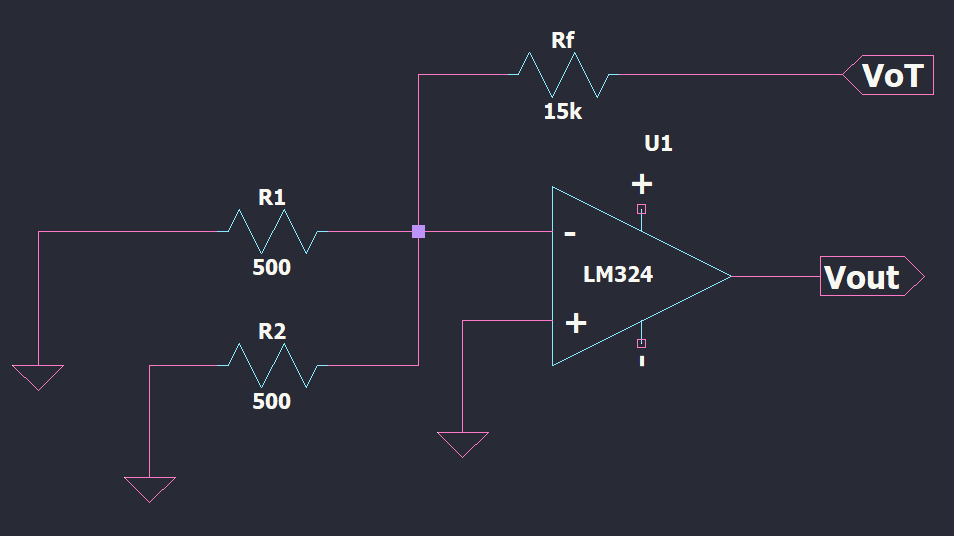
\includegraphics[width=0.90\linewidth]{img/equivalente_lazo.png}
    \caption{Circuito equivalente para el lazo}
    \label{fig:esquematico}
\end{figure}


\[T = \left.\frac{V_{o}}{V_{oT}}\right|_{V_{1}=V_{2}=0} = \frac{V_{o}}{V^{-}} \cdot \frac{V^{-}}{V_{2}} = (-A_d) \frac{(R // R)}{(R // R)+R_f} \]
\[
 T (s) = -Ad(s) \cdot \frac{\frac{R \cdot R}{R+R}}{\frac{R \cdot R}{R+R} + R_f} = ... 
 = -A_d (s) \cdot  \frac{R}{R + 2\cdot R_f}\] 

\subsection{Errores DC}

\subsubsection{Error de corriente de offset: Ios}
Para calcular las corrientes de offset, se pasivan las fuentes y el circuito queda de esta manera:

\begin{figure}[h!]
    \centering
    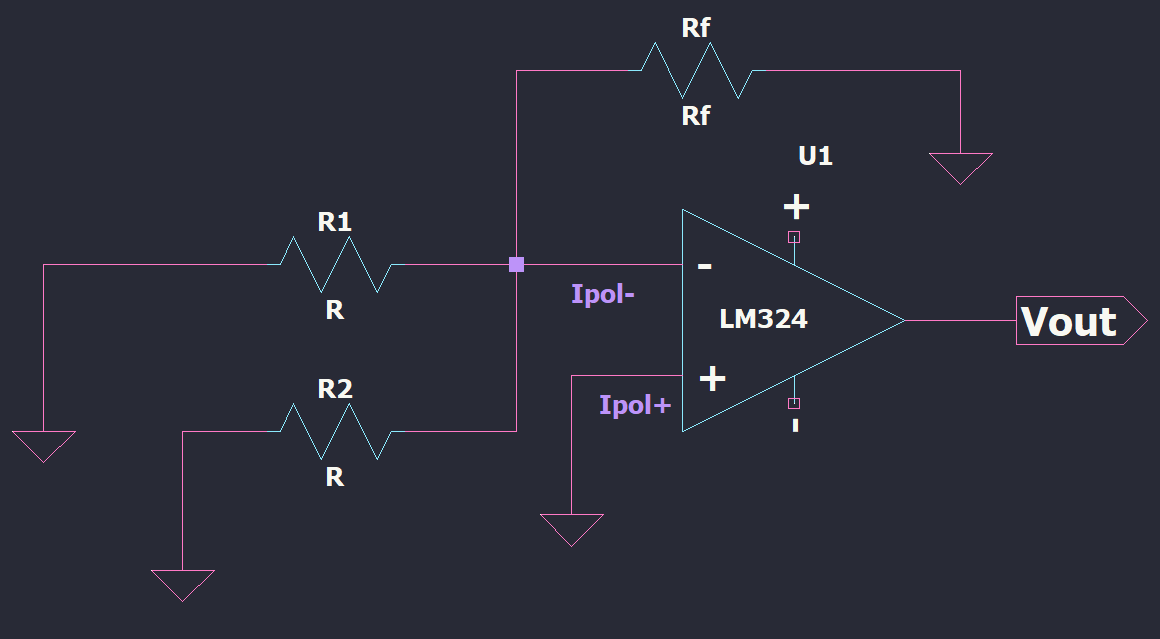
\includegraphics[width=0.90\linewidth]{img/equivalente_ios.png}
    \caption{Circuito equivalente para calcular el error debido a Ipol}
    \label{fig:equivalente_ios}
\end{figure}

\vspace{1em}
Calculamos por partes la ganancia entre la salida y las distintas corrientes de polarización. A continuación se tiene el error debido a la $I_{pol}^{+}$.

\[
\left.\Delta V_{o} \right|_{I_{p o l}^{+}}= I_{p o l}^{+} \cdot R^{+} = 0
\]
Debido a que no hay ninguna impedancia conectada a la entrada no inversora, el error debido a  $I_{pol}^{+}$ es cero.

\vspace{1em}

Luego se tiene el error a lazo abierto debido a la $I_{pol}^{-}$.
 
\[
\left.\Delta V_{o} \right|_{I_{pol}^{+}} = I_{pol}^{-} \cdot (-A_d) \cdot (-R_f // R // R)
\] 

\[\left.\Delta V_{o} \right|_{I_{pol}^{+}} 
= I_{pol}^{-} \cdot (-A_d) \cdot \frac{1}{\frac{1}{R_f}+\frac{1}{R}+\frac{1}{R}} 
= ... = I_{pol}^{-} \cdot A_d \cdot \frac{R_f R}{(R+2 R_f)} \] 
 
Luego si calculamos el error debido a la corriente de offset a lazo cerrado, obtenemos:

 \[ \Delta V_{o_{LA}} = \left.\Delta V_{o} \right|_{I_{pol}^{+}} - \left.\Delta V_{o} \right|_{I_{pol}^{-}}  \] 



\[
\Delta V_{o}= \frac{A_d \frac{R_f R}{(R+2 R_f)} I_{pol}^{-}}{1 - T} 
= \frac{A_d \frac{R_f R}{(R+2 R_f)} I_{pol}^{-}}{1 + A_d \frac{R}{2 R_f+R}} 
= ... =  \frac{Ad \cdot  I_{pol}^{-} \cdot R \cdot R_f}{Ad \cdot R + R + 2 \cdot R_f} 
\] 

Luego  tomando la ganancia ideal del AO $\left(A_{d} \rightarrow \infty\right)$ se cancelan términos y el resultado es:

\[
\Delta V_{o} 
= I_{pol}^{-} \cdot R_f
\]


\subsubsection{Tensión de Offset: Vos}
 
Para el análisis de este error se utiliza el circuito de la figura \ref{fig:equivalentevos}. 


\begin{figure}[h!]
    \centering
    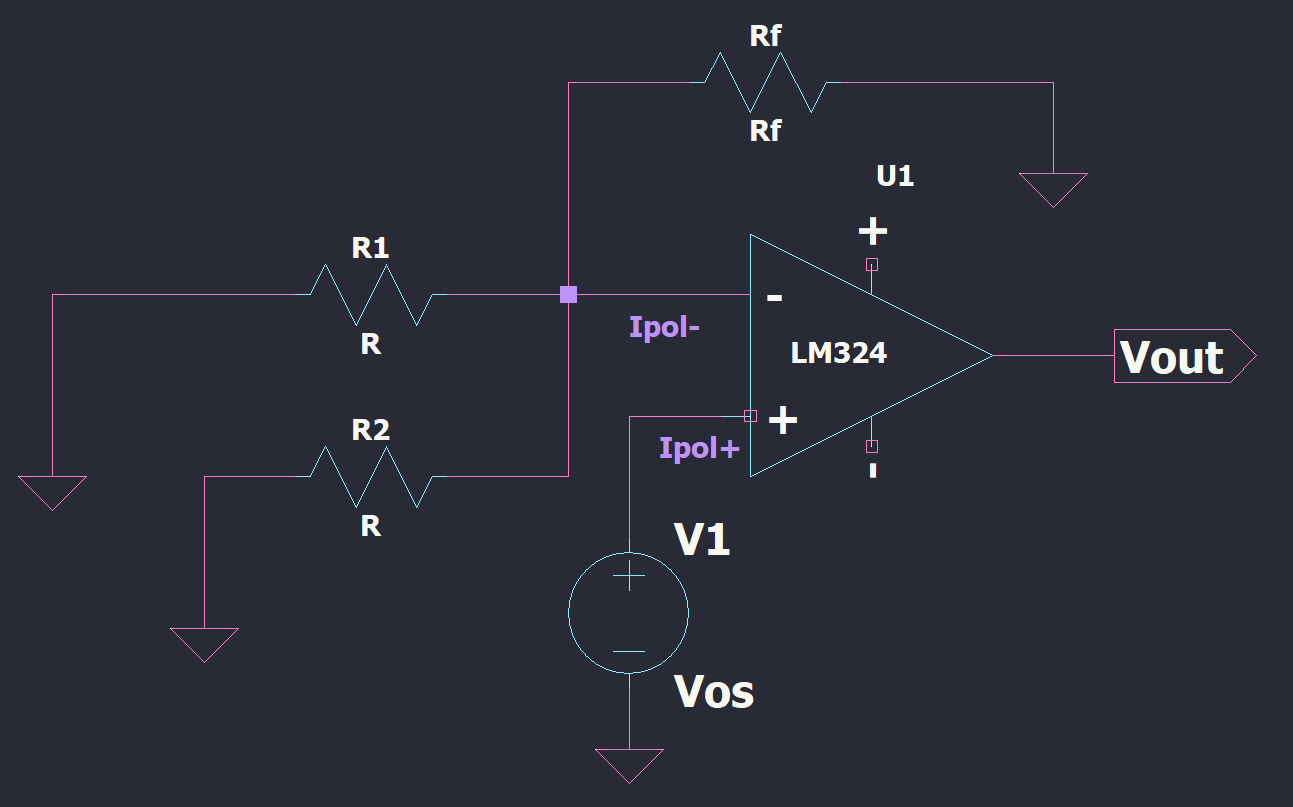
\includegraphics[width=0.90\linewidth]{img/equivalente_vos.png}
    \caption{Circuito equivalente para calcular Vos}
    \label{fig:equivalentevos}
\end{figure}

Se calcula la ganancia de tensión a lazo abierto entre el error $V_{os}$ y la salida.

\[
A_{vos} = \left.\frac{V_{o}}{V_{o s}}\right|_{LA} = 
\frac{V_{o}}{V^{+}} \cdot \frac{V^{+}}{V_{os}} = A_d
\]

Luego si aplicamos black, para obtener el error, se tiene:
 
\[
\Delta V_{os} = \frac{A_d \cdot V_{os}}{1+A_d \frac{R}{2 R_f+R}} = ... 
 = \frac{A_d \cdot V_{os} \cdot (R + 2 \cdot R_f)}{A_d \cdot R + R + 2 \cdot R_f}
\]
 

Como se toma que el amplificador es ideal la ganancia es ideal $\left(A_{d} \rightarrow \infty\right)$ es entonces que se tiene:

\[
\Delta V_{os}  = V_{os} \cdot \frac {R + 2 \cdot R_f}{R} 
=  V_{os} \cdot (1 + 2 \cdot \frac {R_f}{R} )
\]
 
\subsubsection{Ad $ <  \infty $}

Debido a que en la realidad $A_d$ es menor a infinito, debemos considerar el error que aporta.

\[ A_v(s) = \left.\frac{V_0}{V_{1,2}}\right|_{V_{oT} = 0}  = -A_d(s) \cdot \frac{R_f}{R + R_f} = -A_d(s) \cdot (1 - K) \]

\[ T(s) = \left.\frac{V_0}{V_{oT}}\right|_{V_{1,2} = 0} = -A(s) \cdot  \frac{R}{R + 2\cdot R_f}= - A_d(s) \cdot K \]

\[ A_{vf}(s) = \frac{A_d(s)}{1 + K A_d(s)} = \frac{ \frac{1}{K} }{1+\frac{1}{K\cdot A_d(s)}}  \]

\[A_{vf}(s) = \frac{A_{vfi}}{1 - \frac{1}{T(s)}}  \quad  \text{con}  \quad  \epsilon_{G(A_d)} = \frac{1}{T} \]


Luego tenemos que:
\[
\epsilon_{G(A_d)} = \frac{(V_{ideal} - V_{real})}{V_{oi}} = \frac{\Delta V_0}{V_{oi}} \quad \rightarrow \quad \Delta V_0 = \epsilon_{G(A_d)} \cdot V_{oi}  
\]



\[
\Delta V_0 = \epsilon_{G(0)} \cdot V_{o\text{max}} 
\]

Si reemplazamos obtenemos que:

$$
\Delta V_{o}=\frac{F.S}{\left|T_{o}\right|}
$$


\subsubsection{RRMC $\le \infty$}

Como la entrada no inversora del amplificador se encuentra directamente conectado a masa el error debido a la RRMC resulta despreciable:

\[ \Delta V_{o (RRMC) }=0 [ mV ]\]


\subsection{Errores AC}

\subsubsection{Ancho de banda de pequeña señal $f_H$}



Ancho de banda de pequeña señal $\left(w_{h}=-3[d B]\right)$

Observando la hoja de datos del amplificador LM324, obtenemos que:
\[f_T = 1 [MHz]\]
 

Luego, sabiendo que el ancho de banda en pequeña señal se puede calcular con la siguiente formula: 
\[ W_H = W_{T} K \]

De donde K es:
\[ K=\frac{R}{R+2 R f}\]

Por lo tanto, reemplazando en la fórmula general,

\[ w_H = w_{T} \cdot \frac{R}{R+2 R_f} \]


\subsubsection{Ancho de banda a plena potencia \(f_{HP} (10 V_{pap})\) } 


Primero obtenemos el Slew Rate, que se refiere a la velocidad máxima a la que el amplificador operacional puede cambiar su salida cuando hay un cambio en la entrada. Se mide como voltaje relativo al tiempo, y la unidad típica utilizada en las hojas de datos es voltios por microsegundo (V/µs):


 \[ S R=0,5[V / \mu S] \] 

Luego, se utiliza la siguiente fórmula para conocer el valor de $f_{Hp}$, despejando de la misma $\omega_{Hp}$.

\[ S R = \omega_{Hp} \hat{V}_{o} = 2 \pi \cdot  f_{1} \cdot  \hat{V}_{o} \]

Es entonces que reemplazando se tiene:
\[ f_{Hp} = \frac{S R}{2 \pi \hat{V}_{o}} = \frac{0.5[V/ \mu \mathrm{S}]}{2 \pi 10[V]} \]
\[ f_{Hp} = 7,957 [\mathrm{kHz}] \]

\subsubsection{Error vectorial }

Primero obtenemos la ganancia normalizada, que se calcula dividiendo la ganancia a lazo cerrado sobre la ganancia a lazo cerrado ideal (sin variación con la frecuencia):

\[ a_{vf} = \frac{A_{vf}}{A{vfi}} = \frac{1}{1 + \frac{s}{\omega_h}} \]

Luego expresamos su modulo y su fase:

\[ |avf| = \frac{1}{\sqrt{\omega^2_s + 1}} \]


\[ \phi = -atan\left(\frac{\omega}{\omega_h}\right) \]

Con estas definiciones, obtenemos el error vectorial:

\[ \varepsilon_v = \frac{a_{vf}} - 1 \]

Y expresamos en términos de modulo y fase:

\[ |\varepsilon_v| = 1 - \frac{1}{\sqrt{\left(\frac{\omega}{\omega_{h}}\right)^2 + 1}} \]

\[ \phi_v = -\arctan\left(\frac{\omega}{\omega_h}\right) + \frac{\pi}{2} \]


\subsubsection{Tabla de error vectorial normalizado}


\subsubsection{Máxima excursión}
El valor máximo de excursión se obtiene dividiendo el fondo de escala sobre la ganancia media:

\[ V_{max}=\frac{F S}{Avfm} =  \pm 0.33[ V ] \]




\subsection{Resumen}

\[V_{0} = V_{01} + V_{02} = - \frac{R_f}{R} \cdot (V_1 + V_2) \]
\[T (s) = -A_d (s) \cdot  \frac{R}{R + 2\cdot R_f}\]


Errores DC

\[ \Delta V_{ios} = I_{pol}^{-} \cdot R_f \]
\[ \Delta V_{os}  = V_{os} \cdot (1 + 2 \cdot \frac {R_f}{R} )\]
\[ \Delta V_{o (Ad)}=\frac{F.S}{\left|T_{o}\right|}\]
\[ \Delta V_{o (RRMC) } = 0 [ mV ]\]
 
Ancho de banda:

\[ w_H = w_{T} \frac{R}{R+2 R_f} \]

\[ f_{Hp}=7,957[\mathrm{kHz}] \]
 


\newpage

\section{Casi 1.a, resistencia interna de la fuente 50 $\Omega$}

Para este caso, las especificaciones indican que la resistencia interna de la fuente de señal es igual a 50 $\Omega$. Por lo tanto, para no cargar la fuente de señal, la impedancia debe ser mucho mayor a este valor, tomamos como criterio que sea 10 veces mas grande.

Luego, los requerimientos de diseño indican que debe tener una ganancia de -30 veces. 
ganancia vo a cada fuente de señal debe ser -30, 

\[ \text { Si: } R_{i}=50 \Omega \Longrightarrow R=10 R_{i}=500 \Omega \]
\[ \text { Si }: \quad A_{vm} =-\frac{R_{f}}{R}=-30 \]
\[ \text { Entonces }: \quad R_{f}=15 k \Omega \]
\vspace{1em}



\begin{figure}[h!]
    \centering
    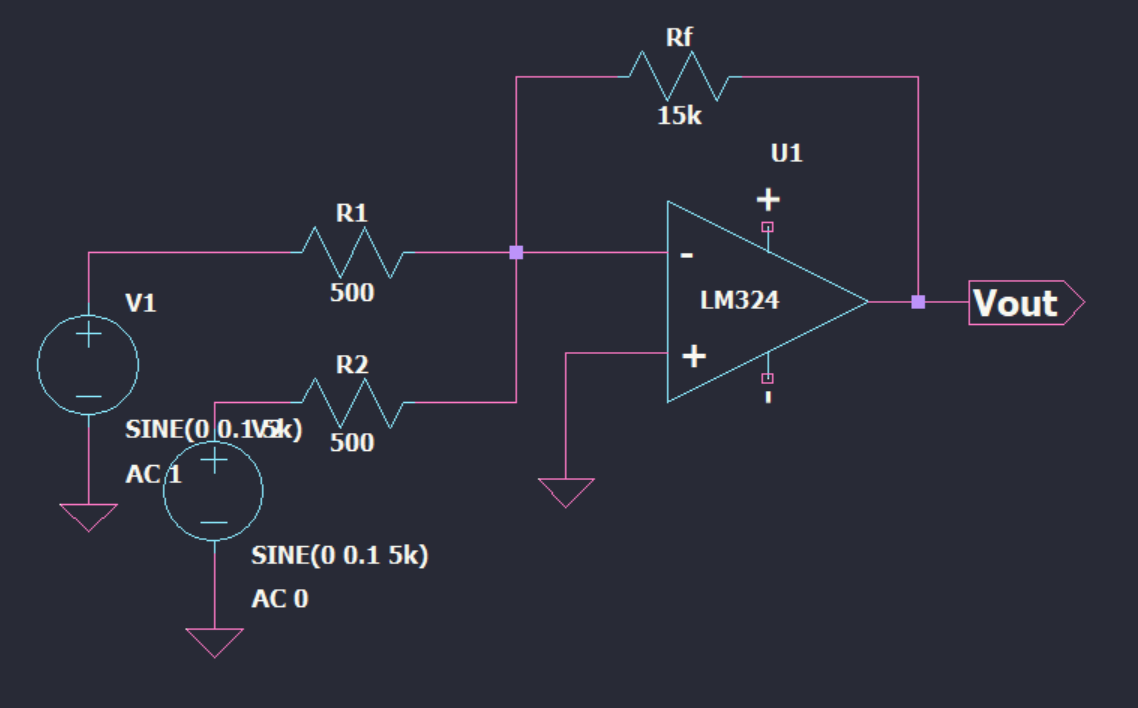
\includegraphics[width=0.90\linewidth]{img/caso1a.png}
    \caption{Esquemático para el caso 1a}
    \label{fig:caso1a}
\end{figure}


\[  \mathbf{R}=500 \Omega, \quad \mathbf{R}_{\mathbf{f}}=15 \mathrm{k} \Omega \]


De esta manera nuestro diseño cumple con las especificaciones de ganancia, impedancia de entrada y valor máximo de resistencias.

\vspace{1em}

\subsection{Errores en DC.}
En primer lugar, obtenemos todos los datos necesarios de la hoja de datos:

\begin{figure}[h!]
    \centering
    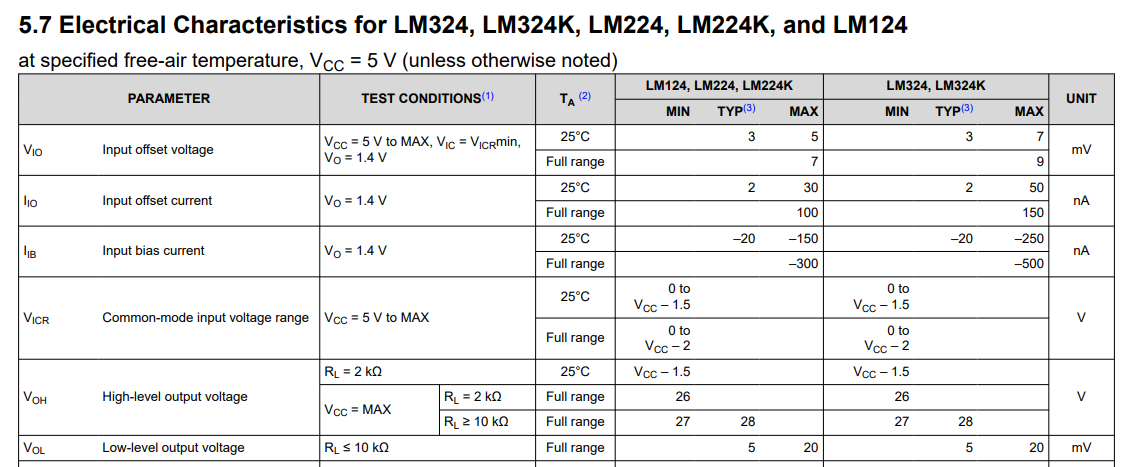
\includegraphics[width=1\linewidth]{img/dc_datasheet.png}
    \caption{Características eléctricas del LM324}
    \label{fig:caracteristicas}
\end{figure}
   
Luego, si reemplazamos por los valores típicos, en las expresiones tenemos que:


\[V_{0} = -30 \cdot (V_1 + V_2) \]
\[T = - Ad   \cdot  \frac{R}{R + 2\cdot R_f} = 100k \cdot \frac{500}{30500} = 1639.3\]

Reemplazando según los datos:
 
\[ \Delta V_{ios} = I_{pol}^{-} \cdot R_f = 20 nF \cdot 15k\Omega = 300 \mu V \]

\vspace{1em}

\[ \Delta V_{os}  = V_{os} \cdot (1 + 2 \cdot \frac {R_f}{R})  =
3mV \cdot 61 = 183 mV \]

\vspace{1em}

\[ \Delta V_{o (Ad)}=\frac{F.S}{\left|T_{o}\right|} = \frac{10V}{1639,39} = 6,1 mV\]

\vspace{1em}

\[ \Delta V_{o (RRMC) } = 0 [ mV ]\]

El error total DC es igual a:

\[ \Delta V_{O} = \Delta V_{ios} + \Delta V_{os} +  \Delta V_{o (A_d)} + \Delta V_{o (RRMC) } = 190 [mV]\]

\subsection{Errores en AC}
 
\subsubsection{Ancho de banda:}

 Primero obtenemos los valores correspondiente a nuestro amplificador de la hoja de datos:

\begin{figure}[h!]
    \centering
    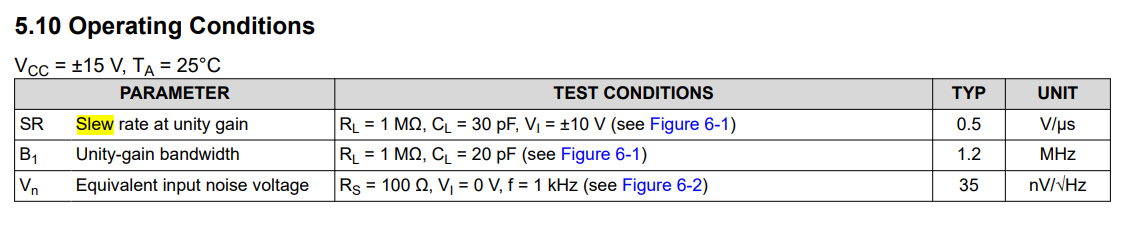
\includegraphics[width=1\linewidth]{img/slewrate_bgw.png}
    \caption{Slew Rate y Producto de ganancia por ancho de banda del LM324}
    \label{fig:slew_rate}
\end{figure}

\[ f_H = f_{T} \frac{R}{R+2 R_f} = 1,2 [MHz] \cdot \frac{500}{30500} = 19,67 [kHz] \]

\subsubsection{Ancho de banda de potencia para 10 $V_{pap}$:}
\[ f_{Hp}=7,957[\mathrm{kHz}] \]


  
 
\subsection { Ganancia normalizada y error vectorial:}
Se analizaron y tabularon los valores de modulo y fase tanto para la ganancia normalizada como para el error vectorial.

\begin{table}[H]
\centering
\begin{tabular}{|c|c|c|c|c|}
\hline
\rowcolor[HTML]{3fb55b} 
$\omega_h$ & \multicolumn{2}{c|}{avf}         & \multicolumn{2}{c|}{Error Vectorial} \\ \cline{2-5} 
\rowcolor[HTML]{3fb55b}  
           & Mod & Fase (°)     &  Mod & Fase (°)  \\ \hline
 (10\%) & 0.99504 & -5.71059 &  0.00496   & 84.28954 \\ \hline
 (20\%) & 0.98058 & -11.30993 &  0.01942  & 78.69    \\ \hline
 (30\%) & 0.95783 & -16.69924 &  0.04217  & 73.3007  \\ \hline
 (40\%) & 0.92848 & -21.80141 &  0.07152  & 68.19859  \\ \hline
 (50 \%)& 0.89443 & -26.56505 &  0.10557  & 63.43502  \\ \hline
 (60 \%)& 0.85749 & -30.96376 &  0.14251  & 59.03642  \\ \hline
 (70 \%)& 0.81923 & -34.99202 &  0.18077  &  55.00795 \\ \hline
 (80 \%)& 0.78087 & -38.65981 &  0.21913  & 51.34045  \\ \hline
 (90 \%)& 0.74329 & -41.98721 &  0.25671  & 48.01271   \\ \hline
 (100 \%) &  0.70711 & -45.0    &   0.29289  & 45.000    \\ \hline 

\end{tabular}
\caption{Ganancia normalizada y error vectorial}
\label{tabla-error}
\end{table}
En la siguiente grafica podemos observar en color ojo al modulo del error vectorial, y luego en azul podemos observar a la fase del error.
El modulo del error aumenta a medida que aumenta la frecuencia, y la fase disminuye.

\begin{figure}[h!]
    \centering
    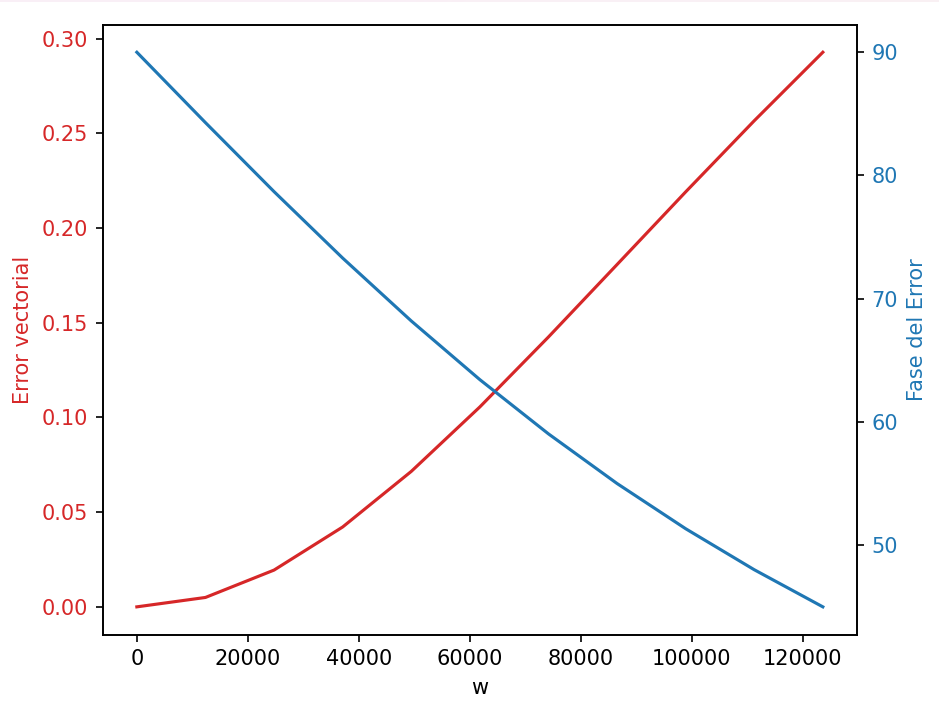
\includegraphics[width=0.80\linewidth]{img/error_vectorial.png}
    \caption{Gráfica error vectorial}
    \label{fig:errorvectorial}
\end{figure}


\newpage
\subsection{Simulaciones}

\subsubsection{Simulación de salida en el tiempo}
 
\begin{figure}[h!]
    \centering
    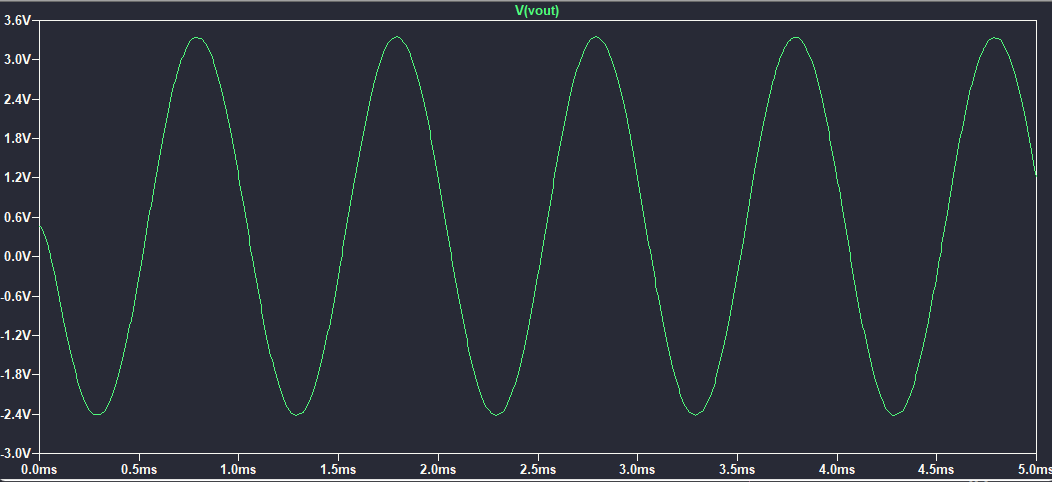
\includegraphics[width=0.80\linewidth]{img/tiempo.png}
    \caption{Gráfico de voltaje de salida en el tiempo}
    \label{fig:tiempo}
\end{figure}

En esta simulación se puede observar que con una entrada de 100 [mV] a 1 [kHz] obtenemos aproximadamente 3[V] de salida


\subsubsection{Simulación de barrido en frecuencia (bode)}
\begin{figure}[h!]
    \centering
    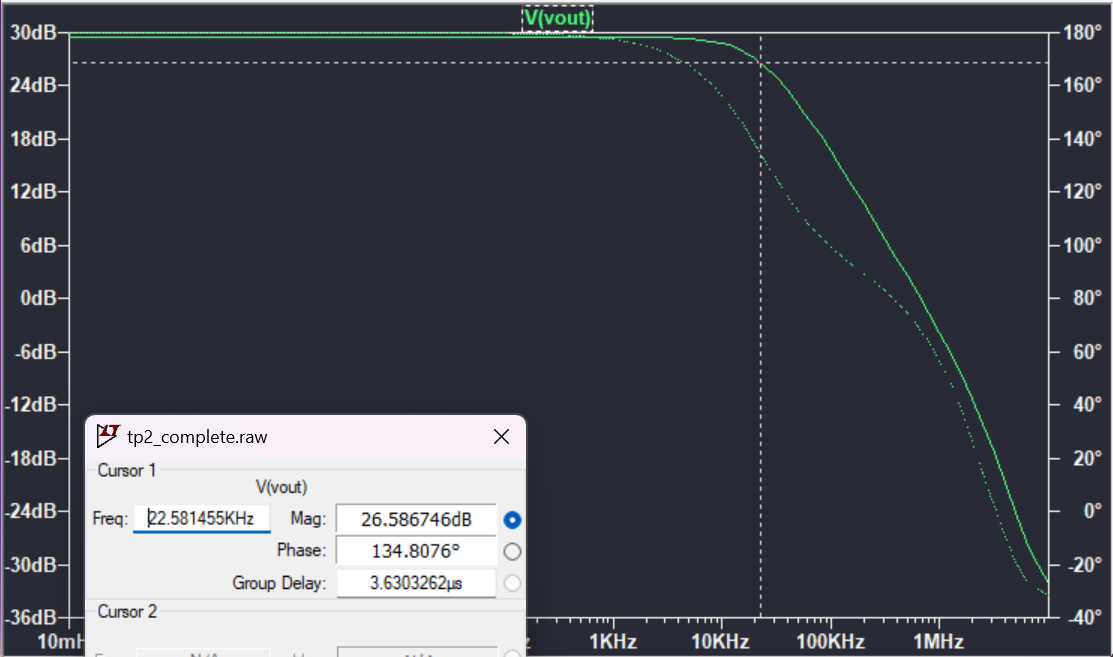
\includegraphics[width=0.80\linewidth]{img/bode1a.png}
    \caption{Gráfico de barrido en frecuencia}
    \label{fig:bode1a}
\end{figure}


\subsubsection{Análisis en frecuencia }

Se pueden observar las armónicas de la señal de salida, frente a una señal de entrada de 1kHz.
\begin{figure}[h!]
    \centering
    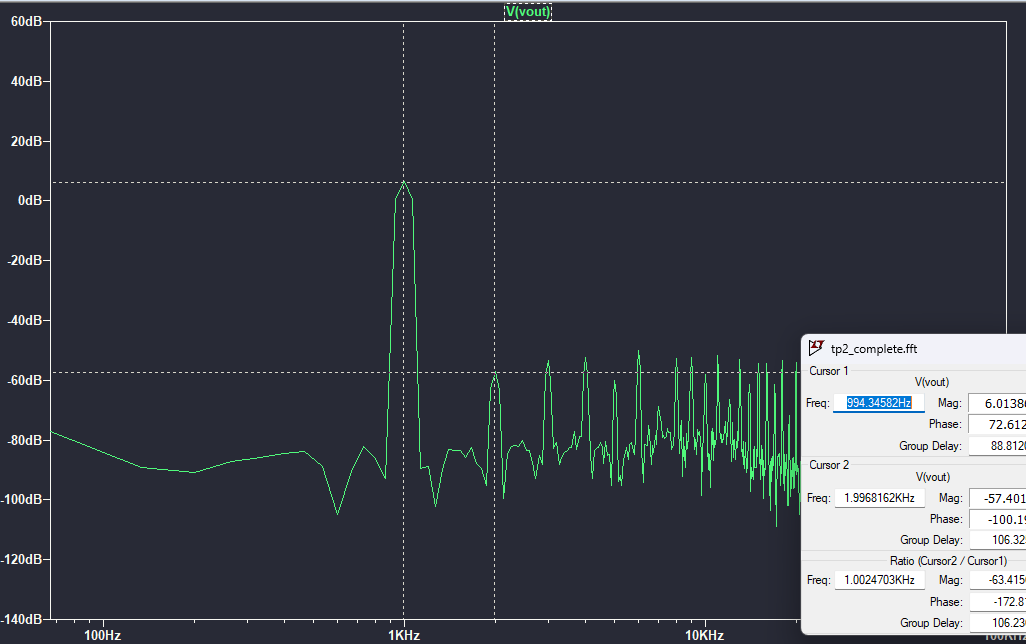
\includegraphics[width=0.80\linewidth]{img/ftt1a.png}
    \caption{Gráfico de la transformada de fourier}
    \label{fig:fft1a}
\end{figure}

\newpage

\section{Caso 1.b, resistencia interna de la fuente 100k $\Omega$}

Para este caso, las especificaciones indican que la resistencia interna de la fuente de señal es igual a 100k $\Omega$. Por lo tanto, para no cargar la fuente de señal, la impedancia debe ser mucho mayor a este valor, tomamos como criterio que sea 10 veces mas grande.

Luego, los requerimientos de diseño indican que debe tener una ganancia de -30 veces. 
ganancia vo a cada fuente de señal debe ser -30, 

\[ \text { Si: } R_{i}=100k \Omega \Longrightarrow R=10 \cdot R_{i} = 1 M\Omega \]
\[ \text { Cumpliendo la condición de }: \quad A_{vm} =-\frac{R_{f}}{R}=-30 \]
\[ \text { Obtenemos }: \quad R_{f}=30 M\Omega \]
Pero esto no cumple con el requerimiento de valor de impedancias menor a 1M $\Omega$
\vspace{1em}

Por lo tanto debemos buscar una manera de obtener una impedancia de realimentación equivalente a 30M $\Omega$ pero solo con resistores menores a 1M$\Omega$.

Hay una forma, desviando utilizando un cuadripolo en ``T'' como realimentación y obtener el mismo resultado:


\begin{figure}[h!]
    \centering
    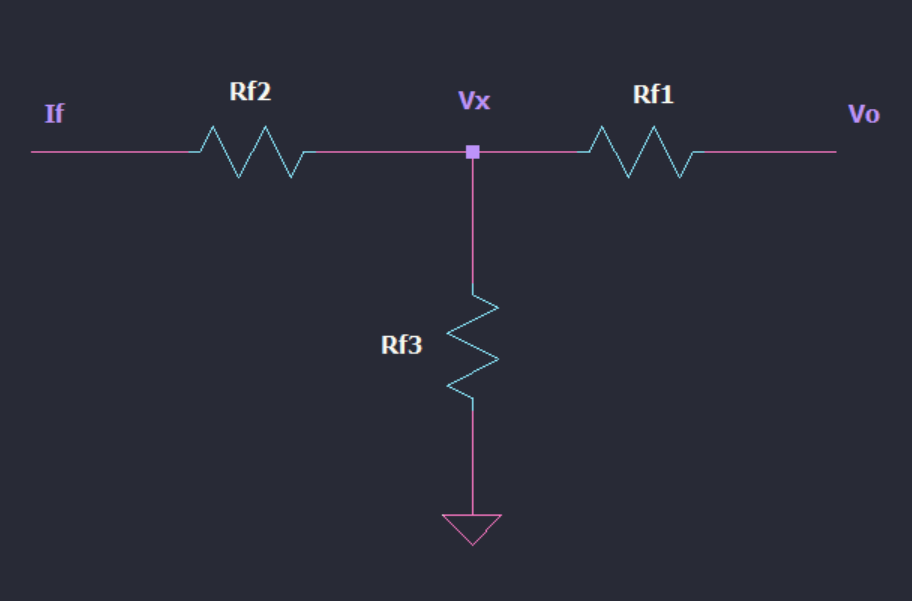
\includegraphics[width=1\linewidth]{img/cuadripoloT.png}
    \caption{Cuadripolo T equivalente a Rf}
    \label{fig:cuadripoloT}
\end{figure}

La impedancia de realimentación equivalente es igual a 

\[Rf = \frac{V_o}{I_f}\]

Para simplificar el calculo, vamos a considerar AO ideal, por lo que la entrada inversora va a ser igual a 0[V].

Luego podemos calcular Vx como la tensión sobre $R_{f3}$:

\[ V_x = \frac{  R_{f2} //  R_{f3} }{ R_{f2} //  R_{f3} + R_{f1} } V_0  = ... = \frac{R_{f2} R_{f3}}{R_{f1} (R_{f2} + R_{f3}) + R_{f2} R_{f3}} \cdot V_o
\]

Con la tensión $V_x$ podemos calcular la corriente $I_f$:

\[ I_f = \frac{V_x}{R_{f2}} = \frac{R_{f3}}{R_{f1} (R_{f2} + R_{f3}) + R_{f2} R_{f3}} \cdot V_o\]


Luego con esto podemos encontrar la impedancia $R_f$:

\[R_f = \frac{V_0}{V_x} \cdot \frac{V_x}{I_f} = \frac{R_{f1} (R_{f2} + R_{f3}) + R_{f2} R_{f3}}{R_{f3}} \]

\[R_f = \frac{R_{f1} \cdot R_{f2} }{R_{f3} } +R_{f1}  + R_{f2}  \]

Por medio de un método iterativo, y variando los valores de $R_{f1}$ y $R_{f2}$ se calcula un valor para $R{f3}$. Teniendo en cuenta valores normalizados de resistores.

\vspace{1em}

Como $R_f = 30M\Omega$ entonces elegimos un valor de $R_{f1} = 390k \Omega$ , $R_{f2} = 91k \Omega$ entonces calculamos:

\vspace{1em}
\[R_{f3} = 1202k\Omega \approxeq 1,2k \Omega \]


\begin{figure}[h!]
    \centering
    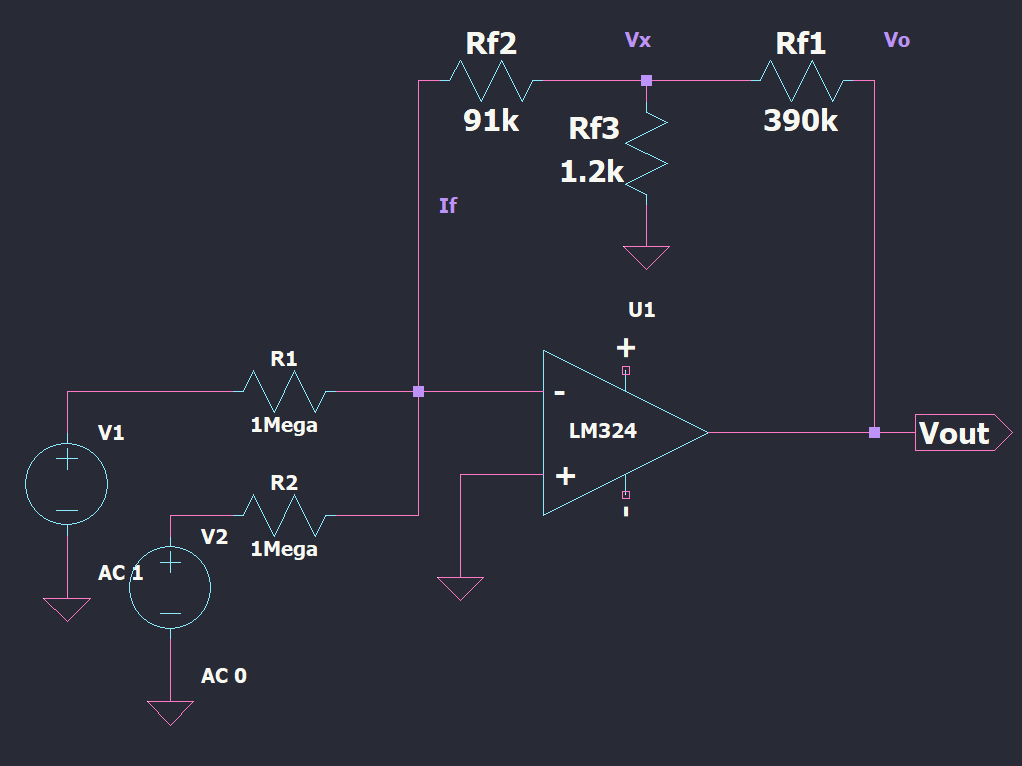
\includegraphics[width=0.90\linewidth]{img/caso1b.png}
    \caption{Esquemático para el caso 1b}
    \label{fig:caso1a}
\end{figure}


\[  \mathbf{R}=1M \Omega, \quad \mathbf{R}_{\mathbf{f}}=30M \mathrm{k} \Omega \]


De esta manera nuestro diseño cumple con las especificaciones de ganancia, impedancia de entrada y valor máximo de resistencias.

\vspace{1em}

\subsection{Errores en DC.}
En primer lugar, obtenemos todos los datos necesarios de la hoja de datos de la figura \ref{fig:caracteristicas}.

\vspace{1em}

Reemplazamos por los valores típicos, en las expresiones tenemos que:


\[V_{0} = -30 \cdot (V_1 + V_2) \]

Luego debemos recalcular T:

\[T = - Ad   \cdot  \frac{R \cdot R_{f3}}{ 2 \cdot (\frac{R}{2} + R_{f2})\cdot (R_{f1}+R_{f3})} = 3114,2 \]


\vspace{1em}

Para realizar los demás cálculos , consideramos a $R_{eq} = R_{f2} + R_{f3}//R_{f1} \approxeq 92k \Omega$
 
\[ \Delta V_{ios} = I_{pol}^{-} \cdot R_{eq} = 20 nF \cdot 92 k\Omega = 1,84 mV \]

\vspace{1em} 

\[ \Delta V_{os}  = V_{os} \cdot (1 + 2 \cdot \frac {R_{eq}}{R})  \approxeq
3mV \cdot 1,18 = 3,553 mV \]

\vspace{1em}

\[ \Delta V_{o (Ad)}=\frac{F.S}{\left|T_{o}\right|} = \frac{10V}{3114,2} = 0,8 mV\]

\vspace{1em}

\[ \Delta V_{o (RRMC) } = 0 [ mV ]\]

El error total DC es igual a:

\[ \Delta V_{O} = \Delta V_{ios} + \Delta V_{os} +  \Delta V_{o (A_d)} + \Delta V_{o (RRMC) } = 6,19 [mV]\]


\subsection{Errores en AC}
 
\subsubsection{Ancho de banda:}

 Primero obtenemos los valores correspondiente a nuestro amplificador de la hoja de datos. Luego
 
\[ f_H = f_{T} \frac{R}{R+2 R_f} = 1,2 [MHz] \cdot \frac{500}{30500} = 19,67 [kHz] \]

\subsubsection{Ancho de banda de potencia para 10 $V_{pap}$:}
\[ f_{Hp}=7,957[\mathrm{kHz}] \]

  
 
\newpage

\subsection{Simulaciones}
\subsubsection{Simulación de salida en el tiempo}
 
\begin{figure}[h!]
    \centering
    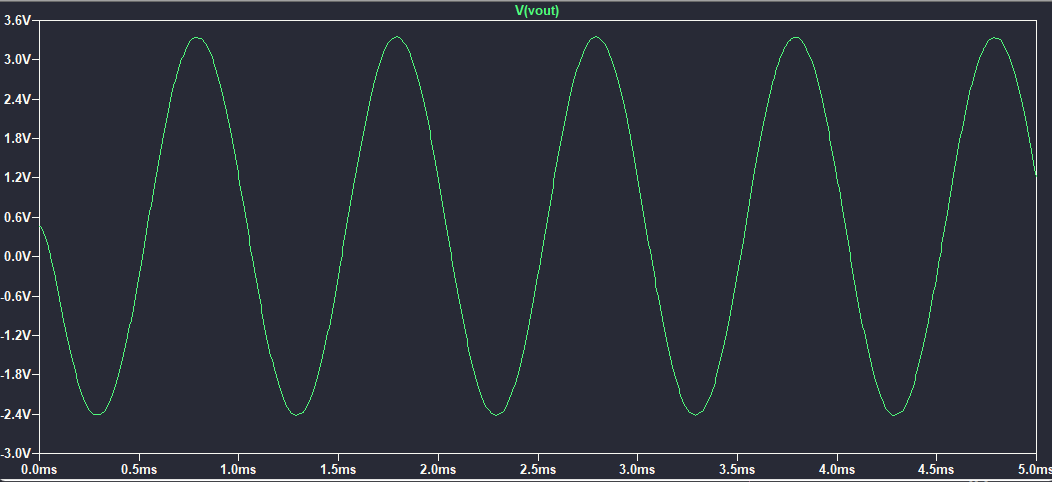
\includegraphics[width=0.80\linewidth]{img/tiempo.png}
    \caption{Gráfico de voltaje de salida en el tiempo}
    \label{fig:tiempo}
\end{figure}

En esta simulación se puede observar que con una entrada de 100 [mV] a 1 [kHz] obtenemos aproximadamente 3[V] de salida. Al igual que la tensión de offset que tiene, ya que no inicia exactamente en 0[V].

\subsubsection{Simulación de barrido en frecuencia (bode)}
\begin{figure}[h!]
    \centering
    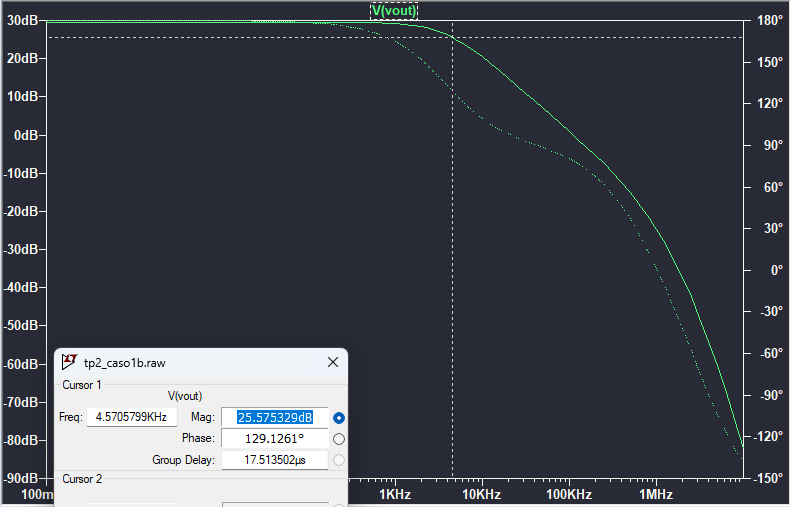
\includegraphics[width=0.80\linewidth]{img/bode.png}
    \caption{Gráfico de barrido en frecuencia}
    \label{fig:bode}
\end{figure}

\subsubsection{Análisis en frecuencia }

Se pueden observar las armónicas de la señal de salida, frente a una señal de entrada de 1kHz.
\begin{figure}[h!]
    \centering
    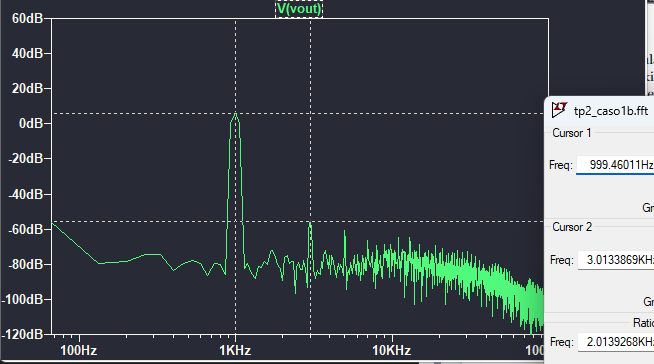
\includegraphics[width=0.80\linewidth]{img/ftt.png}
    \caption{Gráfico de la transformada de fourier}
    \label{fig:fft}
\end{figure}

\subsubsection{Simulación de entrada/salida}

En este caso realizamos un barrido en DC desde -2V a 2V para la fuente de señal $V_1$ y luego se gráfico la tensión de salida $V_o$:

A través de esta simulación se puede observar que la tensión máxima a la que llega la salida es 8,82[V]. Esto se debe a que el amplificador no es Rail to Rail. 

Tambien verificamos que la ganancia es aproximadamente igual a 30 veces.

\begin{figure}[h!]
    \centering
    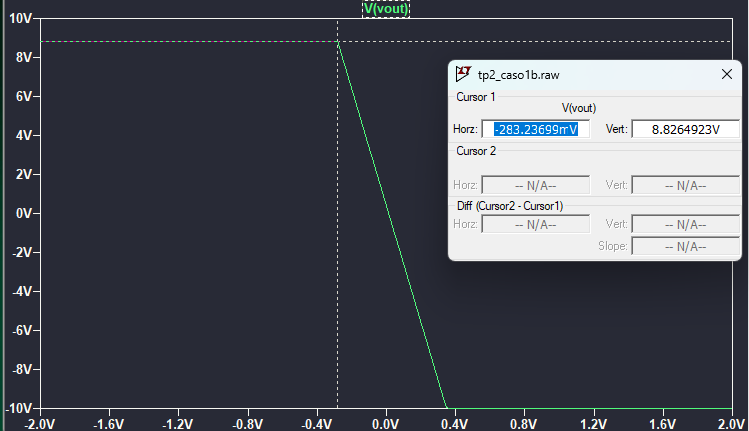
\includegraphics[width=0.80\linewidth]{img/vo_vi.png}
    \caption{Gráfico Vo con respecto a Vi}
    \label{fig:vo_vi}
\end{figure}

\vspace{1em}

\subsubsection{Simulación del Slew rate }

Para esta simulación se puso como entrada una señal cuadrada con tiempo de subido de 1[pS], periodo de 1 [mS] y dutty cycle del 50\%. 

\begin{figure}[h!]
    \centering
    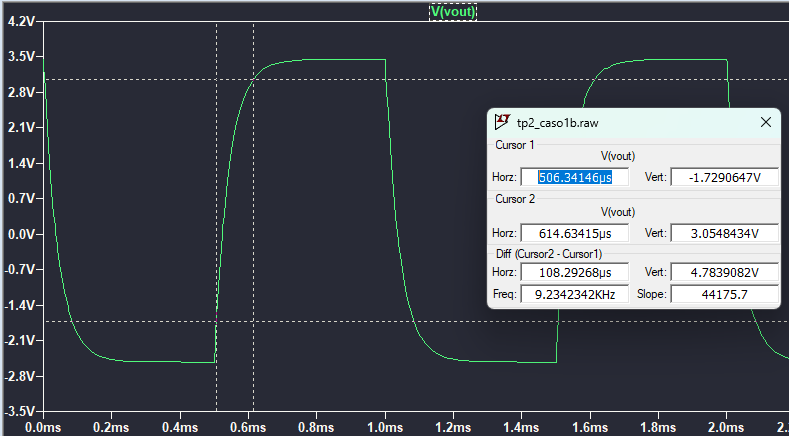
\includegraphics[width=0.90\linewidth]{img/slew_rate.png}
    \caption{Gráfico del slew rate}
    \label{fig:slew_rate}
\end{figure}



\newpage
 


\end{document}
